\subsubsection{Cost function}\label{costfunction}

For the model to learn, it is first necessary to be able to identify errors in the process. The cost function is a function that will calculate the error that is occurring in a model. This function will have two parameters: The expected value and the value calculated by the model. The difference between both values is what is known as error or loss, so this function is also known as loss function or objective function.
\newline

The simplest error is the error given by the difference between the expected value and the actual value:
\newline
\begin{equation}
    \begin{split}
    c_i & = Real_{value} - Expected_{valuue} = \hat{y_i} - y_i, \\ 
    \text{where}~c_i &= \text{The value of the sample loss} \\
    i &= \text{i\textsuperscript{th} sample of the dataset} \\
    ~\hat{y_i} &= \text{Result of the model} \\
    ~y_i &= \text{Real value}
  \end{split}
\end{equation}

Using the example seen before in the regression of figure \ref{fig:regression} the error for the data $i$ seen graphically would be as follows:

\begin{figure}[H]
    \centering
    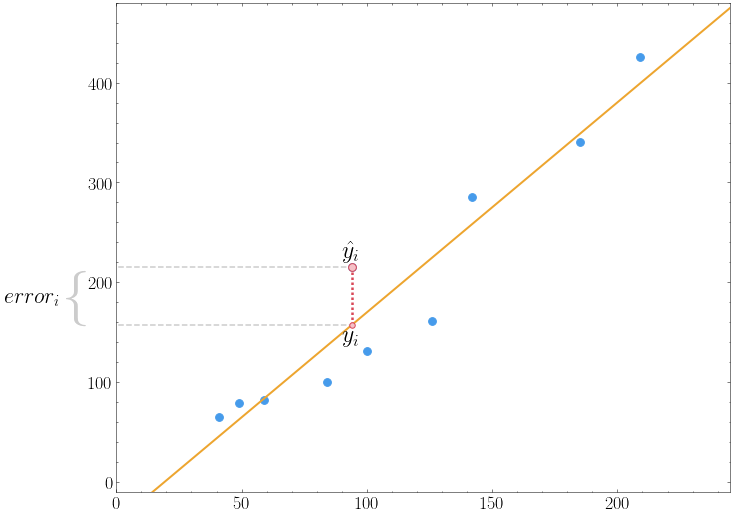
\includegraphics[width=10cm]{images/state-of-art/cost-function/error_function.png}
    \caption{Regression error for data $i$}
    \label{fig:error_regression}
\end{figure}

In a network you need to know the error of the layer and not the error of each neuron. To do this some function will be applied that receives a vector as input (the errors of each neuron in a layer) and a single output value (layer error). Some of the most commonly used functions are listed below \cite{tensorflow2015-whitepaper}:


\begin{itemize}
\item \acrfull{mae} \cite{errors_basics} \label{MAE_loss}: This is the simplest regression error metric to understand. The absolute error of each data is taken, so that negative and positive errors are not cancelled out. Then the arithmetic mean is calculated. In fact, the \acrshort{mae} describes the typical magnitude of the residuals. The equation is as follows:

\begin{equation}
\centering
    \begin{split}
        \text{\acrshort{mae}} = c_i(y_1, \hat{y_1}) = \frac{1}{n} \sum_{i=1}^n |y_i - \hat{y_i}|
    \end{split}
\end{equation}

\begin{figure}[H]
    \centering
    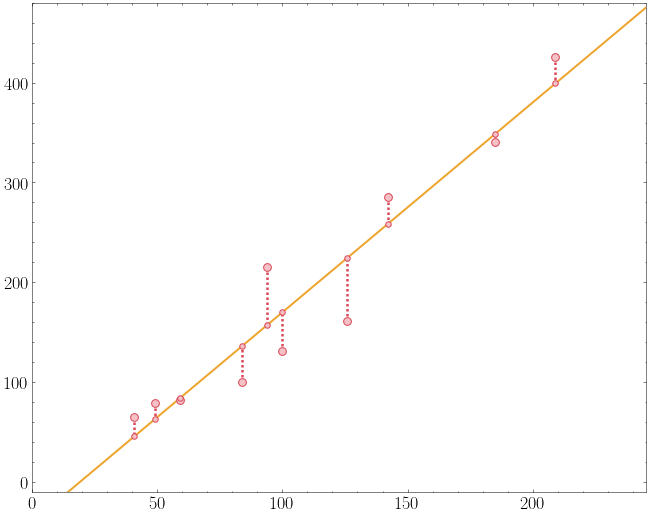
\includegraphics[width=7cm]{images/state-of-art/cost-function/mae.png}
    \caption{Visualisation of the \acrshort{mae}. The error is the arithmetic mean of all errors.}
    \label{fig:error_mae}
\end{figure}

\item \acrfull{mse} \cite{errors_basics}\label{MSE_loss}: This equation calculates the average of all squared errors. By squaring it is possible to penalise with greater intensity those points that are further away from the estimation of the linear regression and with less intensity those that are closer. This equation is widely used when the task to be solved is of a regression type. The equation is as follows:
\begin{equation}
\centering
    \begin{split}
        \text{\acrshort{mse}} = c_i(y_1, \hat{y_1}) &= \frac{1}{n} \sum_{i=1}^n (\sqrt{(\hat{y_i} - y_i)^2}^2) \\
        & = \frac{1}{n} \sum_{i=1}^n (\hat{y_i} - y_i)^2
    \end{split}
\end{equation}

\begin{figure}[H]
    \centering
    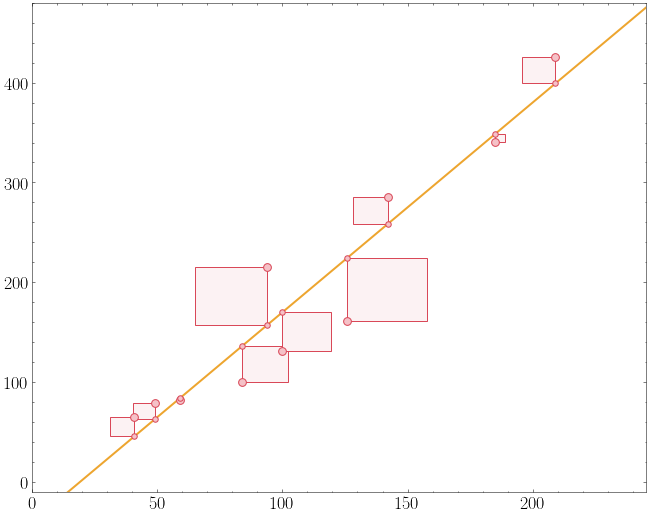
\includegraphics[width=7cm]{images/state-of-art/cost-function/mse.png}
    \caption{Visualisation of the \acrshort{mse}. The error is the average of the areas of the squares.}
    \label{fig:error_mae}
\end{figure}

\item \acrfull{rmse} \cite{errors_basics} \label{RMSE_loss}: This equation is the square root of \acrshort{mse}. If compared at the value level, they are interchangeable although they use different scales. The equation is as follows:
\begin{equation}
\centering
    \begin{split}
        \text{\acrshort{rmse}} = \sqrt{\text{\acrshort{mse}}} = \sqrt{\frac{1}{n} \sum_{i=1}^n (\hat{y_i} - y_i)^2}
    \end{split}
\end{equation}

\item \acrfull{msle} \cite{errors_basics} \label{MSLE_loss}: This equation is similar to \acrshort{mse}. It is often used when it is known in advance that the results are normally distributed and large errors are not intended to be significantly more penalised than small ones. The equation is as follows:
\begin{equation}
\centering
    \begin{split}
        \text{\acrshort{msle}} = c_i(y_1, \hat{y_1}) &= \frac{1}{n} \sum_{i=1}^n (\log{y_i + 1} - \log{\hat{y_i} + 1}) \\
        & = \frac{1}{n} \sum_{i=1}^n \left(\log{\left(\frac{y_i + 1}{\hat{y_i} + 1}\right)}\right)^2
    \end{split}
\end{equation}


\item Huber loss \cite{huber_loss}\label{huber_loss}: It is already known that \acrshort{mse} is better for learning outliers in the data set, on the other hand, \acrshort{mae} is good for ignoring outliers. But in some cases, data that appear to be outliers do not bother and should not be given high priority. The loss of Huber is a combination of \acrshort{mse} and \acrshort{mae}. $\delta$ will be used to define a bias for using \acrshort{mse} or \acrshort{mae}. The equation is as follows:

\begin{equation}
\centering
    \begin{split}
    \text{Huber\_loss} = c_i(y_1, \hat{y_1}) &= \left\{ 
        \begin{array}{cl} 
            \text{\acrshort{mse}} & \text{if }|\hat{y}-y| \le \delta, \\
            \text{\acrshort{mae}} & \text{e.o.c.}
        \end{array}\right. \\ &= \left\{ 
        \begin{array}{cl} 
            \frac{1}{n} \sum_{i=1}^n (\hat{y_i} - y_i)^2 & \text{if }|\hat{y}-y| \le \delta, \\
            \delta \left(\frac{1}{n} \sum_{i=1}^n |y_i - \hat{y_i}|-\frac{\delta}{n}\right) & \text{e.o.c.}
        \end{array}\right.
    \end{split}
\end{equation}

\begin{figure}[H]
    \centering
    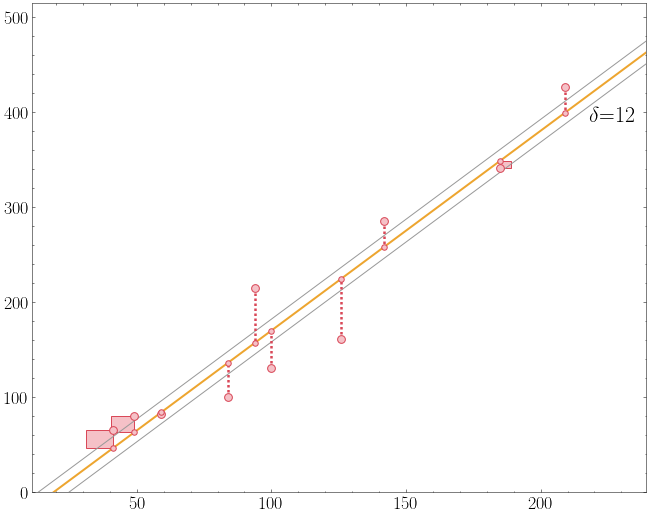
\includegraphics[width=7cm]{images/state-of-art/cost-function/huber.png}
    \caption{Visualisation of Huber loss \acrshort{mse} is calculated if $|\hat{y}-y| \le \delta$, in other
case is calculated \acrshort{mse}.}
\label{fig:error_mae}
\end{figure}


\item \acrfull{mape} \cite{errors_basics} \label{MAPE_loss}: This is the equivalent percentage of \acrshort{mae}. The equation is equal to the \acrshort{mae}, but with adjustments to convert the values into percentages. They allow to see the distance between the model results and the real result showing the data in an easier way to interpret for human beings. The equation is as follows:

\begin{equation}
\centering
    \begin{split}
        \text{\acrshort{mape}} = c_i(y_1, \hat{y_1}) &= \frac{100\%}{n} \sum_{i=1}^n \left|\frac{y_i-\hat{y_i}}{y}\right|
    \end{split}
\end{equation}

\begin{figure}[H]
    \centering
    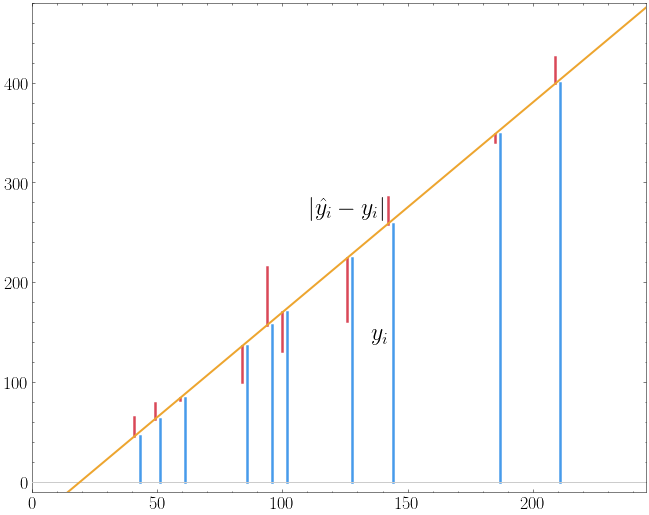
\includegraphics[width=7cm]{images/state-of-art/cost-function/mape.png}
    \caption{\acrshort{mape} visualisation. The error is the mean of the error proportions to with respect to the value $y$.}
    \label{fig:error_mae}
\end{figure}

\item \acrfull{mpe} \cite{errors_basics} \label{MPE_loss}: This is exactly what \acrshort{mape} is, but without the absolute value. Since positive and negative errors are cancelled out, no statement can be made about the overall performance of the model's predictions. However, if there are more negative or positive errors, this bias will be shown in the \acrshort{mpe}. Unlike \acrshort{mape} and \acrshort{mae}, the \acrshort{mpe} is useful because it allows one to see whether the model systematically underestimates (more negative errors) or overestimates (positive errors). The equation is as follows:

\begin{equation}
\centering
    \begin{split}
        \text{\acrshort{mpe}} = c_i(y_1, \hat{y_1}) &= \frac{100\%}{n} \sum_{i=1}^n \frac{y_i-\hat{y_i}}{y}
    \end{split}
\end{equation}

\begin{figure}[H]
    \centering
    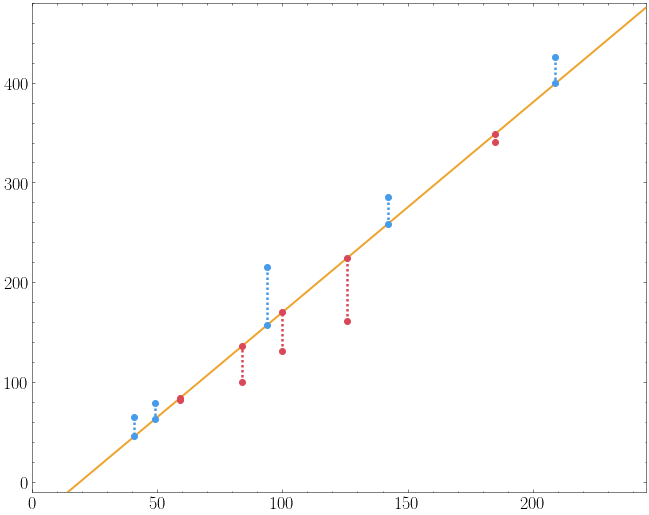
\includegraphics[width=7cm]{images/state-of-art/cost-function/mpe.png}
    \caption{Visualisation of the \acrshort{mpe}. It shows the number of errors that are positive and the number that are negative.}
    \label{fig:error_mae}
\end{figure}


\item Loss of cross entropy: Used explicitly to compare a probability of "fundamental truth" ($y$ or "targets") and some predicted distribution ($\hat{y}$ or "predictions"). It aims to calculate the average of the probabilities that a value belongs to one class or another, so it is very useful for classification problems. It is widely used when the softmax activation function is used, since it also works with probabilities.
\begin{equation}
\centering
    \begin{split}
        c_i(y_1, \hat{y_1}) &= - \sum_i y_{i,j}log(\hat{y_{i,j}})\\
        \text{where}~j &= \text{"True" probability index}
    \end{split}
\end{equation}


The "true" probability is a vector with all values at $0$ except one that has the value equal to $1$. This type of vector is known as an one-hot vector, where a value is hot if it is equal to $1$ or cold if it is equal to $0$. When the results of the model are compared with a one-hot vector using the cross entropy, the values equal to $0$ are not used, and the log loss of the target probability is multiplied by $1$, making the calculation of cross entropy relatively simple. This is also a special case of the calculation of cross entropy, called category cross entropy.
\newline

An example of a one-hot vector would be the following: $[0,1,0,0]$ where for example the following classes would be represented: Dog, cat, horse and elephant. The $1$ represents that the data given to the model represents a cat. These types of vectors are widely used in classification tasks and in \acrfull{nlp}.
\newline

There is a subtype called binary cross entropy loss. This type of error can be calculated when trying to classify only with two types: $0$ or $1$. It is usually used as if it were a boolean value in a programming language. A \small{\verb|true|} \normalsize if it is type A or a \small{\verb|false|} \normalsize if it is not type A. For example: cat or no cat or indoor or outdoor. The mathematical equation is as follows:

\begin{equation}
\centering
    \begin{split}
        c_{i,j}(y_1, \hat{y_1}) &= (y_{i,j})(-log(\hat{y}_{i,j})) + (1-y_{i,j}) (-log(1 - \hat{y}_{i,j})) \\
        &= -y_{i,j} \cdot log(\hat{y}_{i,j}) - (1 - y_{i,j}) \cdot log(1 - \hat{y}_{i,j})
    \end{split}
\end{equation}


\end{itemize}

